% -*- latex -*-
%%%%%%%%%%%%%%%%%%%%%%%%%%%%%%%%%%%%%%%%%%%%%%%%%%%%%%%%%%%%%%%%
%%%%
%%%% This TeX file is part of the course
%%%% Introduction to Scientific Programming in C++/Fortran2003
%%%% copyright 2017-2022 Victor Eijkhout eijkhout@tacc.utexas.edu
%%%%
%%%% array.tex : basic language elements
%%%%
%%%%%%%%%%%%%%%%%%%%%%%%%%%%%%%%%%%%%%%%%%%%%%%%%%%%%%%%%%%%%%%%

An \indextermdef{array}\footnote
{The term `array' is used informally here.
  There is an \texttt{array} keyword,
  which is briefly discussed in section~\ref{sec:cpp-array}.}
is an indexed data structure that for each
index stores an integer, floating point number, character,
object, et cetera.
In scientific applications, arrays often correspond to vectors and
matrices, potentially of quite large size. (If you know about the
\acf{FEM}, you know that vectors can have sizes in the millions or beyond.)

In this chapter you will see the C++ \indexc{vector} construct,
which implements the notion of an array of things, whether they be
numbers, strings, objects.

\begin{slide}{What are vectors?}
  \label{sl:what-vector}
  \begin{itemize}
  \item Contiguous, indexed, storage of items:\\
    (often called `array' but that has other meanings)
    \begin{itemize}
    \item items of any type (but the same for all elements of one
      vector)
    \item potentially very many items
    \end{itemize}
  \item Indexed set of items
  \item \ldots~but if you don't need the index: collection of items
  \end{itemize}
\end{slide}

\begin{cnote}
  While C++ can use the C~mechanisms for arrays, for almost all purposes
  it is better to use \lstinline{vector}. In particular, this is a safer way to
  do dynamic allocation. The old
  mechanisms are briefly discussed in section~\ref{sec:staticarray}.
\end{cnote}

\begin{slide}{Vectors are better than arrays}
  \label{sl:vector-why}
  Vectors are fancy arrays. They are easier and safer to use:
  \begin{itemize}
  \item They know what their size is.
  \item Bound checking.
  \item Freed when going out of scope: no memory leaks.
  \item Dynamically resizable.
  \end{itemize}
  In C++ you never have to \indexc{malloc} again.\\
  (Not even \indexc{new}.)
\end{slide}

\Level 0 {Some simple examples}

\Level 1 {Vector creation}

To use vectors, you first need the \lstinline{vector} header from the \ac{STL}.
This allows you to declare a vector, specifying what type of element
it contains. Next you may want to decide how many elements it
contains; you can specify this when you declare the vector, or
determine it later, dynamically.

We start with the most obvious way of creating a vector:
enumerating its elements.

\begin{block}{Short vectors}
  \label{sl:vectorshort}
  Short vectors can be created by enumerating their elements:
  %
  \verbatimsnippet{shortvectorex}
\end{block}

\begin{exercise}
  \label{ex:shortvectoralter}
  \begin{enumerate}
  \item
    Take the above snippet, supply the missing header lines, compile, run.
  \item Add a statement that alters the value of a vector element.
    Check that it does what you think it does.
  \item Add a vector of the same length, containing odd numbers,
    which are the even values plus~1?
  \end{enumerate}
  \skeleton{shortvector}
\end{exercise}

A more sophisticated example:
\begin{lstlisting}
vector<Point> diagonal = 
    { {0.,0.}, {1.,1.}, {1.5,1.5}, {2.,2.}, {3.,3.} };
\end{lstlisting}

\Level 1 {Initialization}

There are various ways to declare a vector, and possibly initialize it.

More generally, vectors can be defined
\begin{itemize}
\item Without further specification, creating an empty vector:
\begin{lstlisting}
vector<float> some_numbers;
\end{lstlisting}
\item With a size indicated, allocating that number of elements:
\begin{lstlisting}
vector<float> five_numbers(5);
\end{lstlisting}
(This sets the elements to a default value; zero for numeric types.)
\item You can initialize a vector with a constant:
\begin{lstlisting}
vector<float> x(25,3.15);
\end{lstlisting}
which defines a vector \lstinline{x} of size~25,
with all elements initialized to~3.15.
\end{itemize}

\begin{slide}{Vector constant initialization}
  \label{sl:vector-initconst}
  There is a syntax for initializing a vector with a constant:
\begin{lstlisting}
vector<float> x(25,3.15);
\end{lstlisting}
which defines a vector \lstinline{x} of size~25,
with all elements initialized to~3.15.
\end{slide}

If your vector is short enough, you can set all elements explicitly with an
\indextermbus{initializer}{list}, and note that the size is not specified here,
but is deduced from the length of the initializer list:

\snippetwithoutput{dynamicinit}{array}{dynamicinit}

\begin{slide}{Vector initialization}
  \label{sl:vector-init}
  You can initialize a vector as a whole:
  \begin{lstlisting}
    vector<float> halves{ 0.5, 1.5, 2.5, 3.5 };
  \end{lstlisting}
  (Note: no size given)
\end{slide}

\begin{slide}{Vector definition}
  \label{sl:vector-def}
  Definition and/or initialization:
\begin{lstlisting}
#include <vector>
using std::vector;

vector<type> name;
vector<type> name(size);
vector<type> name(size,init_value);
\end{lstlisting}
where
\begin{itemize}
\item \indexc{vector} is a keyword,
\item \n{type} (in angle brackets) is any elementary type or class
  name,
\item \n{name} of the vector is up to you, and
\item \n{size} is the (initial size of the vector). This is an integer,
  or more precisely, a \indexc{size_t} parameter.
\item Initialize all elements to \n{init_value}.
\item If no default given, zero is used for numeric types.
\end{itemize}
\end{slide}

\begin{review}
  T/F? 
  \begin{itemize}
  \item It is possible to write a valid C++ program where you define a
    variable \lstinline+vector+.
  \end{itemize}
\end{review}

\Level 1 {Element access}

There are two ways of accessing vector elements.
\begin{enumerate}
\item With the `dot' notation that you know from structures and objects, 
  you can use the \indexc{at} method:
\snippetwithoutput{assignatfun}{array}{assignatfun}
\item
  There is also a short-hand notation (which is the same as in~C):
\snippetwithoutput{assignbracket}{array}{assignbracket}
\end{enumerate}

Indexing starts at zero. Consequently, a vector declared as
\begin{lstlisting}
vector<int> ints(N)
\end{lstlisting}
has elements $0,\ldots,N-1$.

As you see in this example,
if \lstinline{a}~is a vector, and \lstinline{i} an integer,
then \lstinline+a.at(i)+ is the i'th element.
\begin{itemize}
\item The expression \lstinline+a.at(i)+ can be used to get the value of a
  vector element, or it can occur in the left-hand side of an
  assignment to set the value
\begin{lstlisting}
vector<float> x(25);
x.at(2) = 3.14;
float y = y.at(2);
\end{lstlisting}
\item The same holds for indexing with square brackets.
\begin{lstlisting}
vector<float> x(25);
x[2] = 3.14;
float y = y[2];
\end{lstlisting}
\item The \indextermbus{vector}{index} (or
  \indextermbus{vector}{subscript}) \n{i} starts numbering at zero.
\item Therefore, if a vector has $n$ elements, its last element has
  index~\n{n-1}.
\end{itemize}

\begin{slide}{Accessing vector elements}
  \label{sl:vectorsub}
  Square bracket notation (zero-based):
  \snippetwithoutput{assignbracket}{array}{assignbracket}

  With bound checking:
  \snippetwithoutput{assignatfun}{array}{assignatfun}
  Safer, slower.\\
  (Remember Knuth about optimization.)
\end{slide}

\Level 1 {Access out of bounds}

Have you wondered what happens if you access a
vector element outside the bounds of the vector?
\begin{lstlisting}
vector<float> x(6); // size 6, index ranges 0..5
x.at(6) = 5.; // oops!
i = -2;
x[i] = 3; // also oops, but different.
\end{lstlisting}
Usually, it is hard for the compiler to determine that you are
accessing an element outside the vector bounds.
Most likely, it will only be detected at runtime.
There is now a difference in how the two accessing methods
do \indextermbus{vector}{bounds checking}.

\begin{slide}{Vector elements out of bounds}
  \label{sl:vectorsuboob}
  Square bracket notation:
  \snippetwithoutput{assignbracketoob}{array}{assignoutofboundbracket}

  With bound checking:
  \snippetwithoutput{assignatfunoob}{array}{assignoutofboundatfun}
  Safer, slower.\\
  (Remember Knuth about optimization.)
\end{slide}

\begin{enumerate}
\item Using the \indexc{at} method will always do a bounds test,
  and exit your program immediately if you access an element
  outside the vector bounds.
  (Technically, it throws an \indexterm{exception};
  see section~\ref{sec:exception} for how this works and how you can handle this.)
\item The bracket notation \lstinline{a[i]} performs no bounds tests:
  it calculates a memory address based on the vector location and the index,
  and attempts to return what is there.
  As you may imagine, this lack of checking makes your code a little faster.
  However, it also makes your code unsafe:
  \begin{itemize}
  \item Your program may crash with a \indexterm{segmentation fault}
    or \indexterm{bus error}, but no clear indication where and why this happened.
    (Such a crash can be caused by other things than vector access out of bounds.)
  \item Your program may continue running, but  giving wrong results,
    since reading from outside the vector probably gives you meaningless values.
    Writing outside the bounds of an vector may even change the data of other variables,
    leading to really strange errors.
  \end{itemize}
\end{enumerate}
For now, it is best to use the \indexc{at} method throughout.

\begin{block}{Vector index out of bounds}
  Indexing out of bounds can go undetected for a while:
  
  \snippetwithoutput{vectoroutofbound}{array}{segmentation}
\end{block}

\begin{review}
  The following codes are not correct in some sense. How will this manifest itself?
  %\verbatimsnippet{staterr}
  \verbatimsnippet{vecerr}
  \verbatimsnippet{vecexc}
\end{review}

In some applications you will create an vector, and gradually fill it,
for instance in a loop. However, sometimes your elements are known in
advance and you can write them out. Specifying these values while
creating the vector is called \indextermbus{vector}{initialization}, and
there is more than one way to do so.

First of all, you can set a vector to a constant:

\Level 0 {Going over all vector elements}
\label{sec:arrayrange}

If you need to consider all the elements in a vector, you typically
use a \indexc{for} loop. There are various ways of doing this.

\begin{block}{A philosophical point}
  \label{sl:vector-access-types}

  Conceptually, a \indexc{vector} can correspond to a set of things,
  and the fact that they are indexed is purely incidental,
  or it can correspond to an ordered set,
  and the index is essential.
  If your algorithm requires you to access all elements,
  it is important to think about which of these cases apply,
  since there are two different mechanism.
\end{block}

\Level 1 {Ranging over a vector}

First of all consider the cases where you consider the vector as a
collection of elements, and the loop functions like a mathematical
`for all'.

\index{range-based for loop|see{for, range-based}}
\begin{block}{Range over elements}
  \label{sl:vector-range}
  You can write a \indextermsub{range-based}{for} loop, which
  considers the elements as a collection.
\begin{lstlisting}
for ( float e : my_data )
  // statement about element e
for ( auto e : my_data )
  // same, with type deduced by compiler
\end{lstlisting}
\snippetwithoutput{dynamicmax}{array}{dynamicmax}
\end{block}

(You can spell out the type of the vector element, but such type
specifications can be complex.
In that case, using \indextermbus{type}{deduction}
through the \indexc{auto} keyword
is quite convenient.)

So-called \indextermbus{initializer}{list}s
can also be used as a list denotation:

\begin{block}{Range over vector denotation}
  \label{sl:range-denote}
  \snippetwithoutput{rangedenote}{array}{rangedenote}  
\end{block}

\Level 1 {Ranging over the indices}

If you actually need the index of the element, you can use a
traditional \indexc{for} loop with loop variable.

\begin{block}{Indexing the elements}
  \label{sl:index-range}
  You can write an \indextermsub{indexed}{for} loop, which uses an
  index variable that ranges from the first to the last element.
\begin{lstlisting}
for (int i= /* from first to last index */ )
  // statement about index i
\end{lstlisting}
Example: find the maximum element in the vector, and where it occurs.
%
\snippetwithoutput{vecidxmax}{array}{vecidxmax}
\end{block}

\begin{exercise}
  \label{ex:range-for}
  Indicate for each of the following vector operations whether you
  prefer to use an indexed loop or a range-based loop. Give a short
  motivation.
  \begin{itemize}
  \item Count how many elements of a vector are zero.
  \item Find the location of the last zero.
  \end{itemize}
\end{exercise}

\begin{exercise}
  \label{ex:array-max}
  Find the element with maximum absolute value in a vector. Use:
\begin{lstlisting}
vector<int> numbers = {1,-4,2,-6,5};
\end{lstlisting}
% Which mechanism do you use for traversing the vector?

Hint:
\begin{lstlisting}
#include <cmath>
..
absx = abs(x);
\end{lstlisting}
\end{exercise}

\begin{exercise}
  \label{ex:array-maxidx}
  Find the location of the first negative element in a vector.

  Which mechanism do you use?
\end{exercise}

\begin{exercise}
  \label{ex:array-sorted}
  Check whether a vector is sorted.
\end{exercise}

\Level 1 {Ranging by reference}

\begin{block}{Range over elements by reference}
  \label{sl:vector-range-ref}
  Range-based loop indexing makes a copy of the vector element. If you
  want to alter the vector, use a reference:
  %
\begin{lstlisting}
for ( auto &e : my_vector)
  e = ....
\end{lstlisting}
%
\snippetwithoutput{vectorrangeref}{array}{vectorrangeref}

(Can also use \lstinline{const auto& e} to prevent copying, but also
prevent altering data.)
\end{block}

\begin{exercise}
  If you do the prime numbers project, you can now do exercise~\ref{ex:arraysieve}.
\end{exercise}

In a \indexc{while} loop, if you need an index,
you need to maintain that index explicitly.
There are then certain common idioms.

\begin{block}{Example of increment indexing}
  \label{sl:plusplusexample}
  \snippetwithoutput{plusplustest1}{loop}{plusplus}
\end{block}

\begin{slide}{Indexing with pre/post increment}
  \label{sl:prepostindex}
Indexing in \indexc{while} loop and such:
\begin{lstlisting}
x = a.at(i++); /* is */ x = a.at(i); i++;
y = b.at(++i); /* is */ i++; y = b.at(i);
\end{lstlisting}
\end{slide}

\begin{exercise}
  Exercise: modify the preceeding code so that after the while loop
  \n{index} is the number of leading odd elements.
\end{exercise}

\Level 0 {Vector are a class}
\label{sec:stdvector}

Above, you created vectors and used functions \indexc{at} and \indexc{size}
on them. They used the dot-notation of class methods, and in fact
vector form a \indexcdef{vector} class. You can have a vector of ints,
floats, doubles, et cetera; 
the angle bracket notation indicates what the specific type stored in
the vector is.
You could say that the vector class is parametrized with the type (see
chapter~\ref{ch:template} for the details). We could say that
\lstinline{vector<int>} is a new data type, pronounced `vector-of-int', and you can
make variables of that type.

\begin{block}{Vector copy}
  \label{sl:vectorcopy}
  Vectors can be copied just like other datatypes:
  %
  \snippetwithoutput{vectorcopy}{array}{vectorcopy}
\end{block}

\Level 1 {Vector methods}

There are several \emph{methods}\index{vector!methods}
to the \lstinline{vector} class. Some of the simpler ones are:
\begin{itemize}
\item \indexc{at}: index an element
\item \indexc{size}: give the size of the vector
\item \indexc{front}: first element
\item \indexc{back}: last element
\end{itemize}

There are also methods relating to dynamic storage management, which
we will get to next.

\begin{exercise}
  \label{ex:vectornormalize}
  Create a \n{vector} $x$ of \lstinline{float} elements, and set them to random
  values. (Use the C random number generator for now.)

  Now normalize the vector in $L_2$ norm and check the correctness of
  your calculation, that is,
  \begin{enumerate}
  \item Compute the $L_2$ norm of the vector:
    \[ \| v\| \equiv \sqrt{\sum_iv_i^2} \]
  \item Divide each element by that norm;
  \item The norm of the scaled vector should now by~1. Check this.
  \item Bonus: your program may be printing~1, but is it actually~1?
    Investigate.
  \end{enumerate}
  What type of loop are you using?
\end{exercise}


\begin{slide}{Vector methods}
  \label{sl:vector-method}
  A vector is an object, with methods.

  Given \lstinline+vector<sometype> x+:
  \begin{itemize}
  \item Get elements, including bound checking, with
    \lstinline{ar.at(3)}.
    Note: (zero-based indexing).
  \item (also get elements with \lstinline{ar[3]}: see later discussion.)
    %% (for C programmers: this is not dereferencing, this uses an
    %% operator method)
  \item Size: \lstinline{ar.size()}.
  \item Other functions: \indexc{front}, \indexc{back}, \indexc{empty}.
  \item With iterators (see later): \indexc{insert}, \indexc{erase}
  \end{itemize}
\end{slide}

\begin{block}{Your first encounter with templates}
  \label{sl:vector-template}
 \lstinline{vector} is a `templated class':
    \lstinline{vector<X>} is a vector-of-\lstinline{X}.

    Code behaves as if there is a class definition for each type:
    \begin{multicols}{2}
      \small
\begin{lstlisting}
class vector<int> {
public:
  size(); at(); // stuff
}
\end{lstlisting}
\begin{lstlisting}
class vector<float> {
public:
  size(); at(); // stuff
}
\end{lstlisting}
    \end{multicols}
    Actual mechanism uses templating:
    the type is a parameter to the class definition. More later.
\end{block}

\Level 1 {Vectors are dynamic}
\label{sec:stdvector-dynamic}

A vector
can be grown or shrunk after its creation.
For instance, you can use the \indexc{push_back} method to add elements at the end.

\begin{block}{Dynamic vector extension}
  \label{sl:vector-dynamic}
  Extend a vector's size with \indexc{push_back}:
  %
  \snippetwithoutput{vectorpush}{array}{vectorend}
  %
  Similar functions: \indexc{pop_back}, \indexc{insert}, \indexc{erase}.
  \slidenewline
  Flexibility comes with a price.
\end{block}

It is tempting to use \indexc{push_back} to create a vector dynamically.

\begin{block}{When to push back and when not}
  \label{sl:vecpushnot}
  \begin{multicols}{2}
    Known vector size:
\begin{lstlisting}
int n = get_inputsize();
vector<float> data(n);
for ( int i=0; i<n; i++ ) {
  auto x = get_item(i);
  data.at(i) = x;
}
\end{lstlisting}
\columnbreak
    Unknown vector size:
\begin{lstlisting}
vector<float> data;
float x;
while ( next_item(x) ) {
  data.push_back(x);
}
\end{lstlisting}
  \end{multicols}
  If you have a guess as to size: \lstinline+data.reserve(n)+.
\end{block}

\begin{block}{Dynamic size extending}
  \label{sl:vector-extend}
\begin{lstlisting}
vector<int> iarray;
\end{lstlisting}
creates a vector of size zero. You can then
\begin{lstlisting}
iarray.push_back(5);
iarray.push_back(32);
iarray.push_back(4);
\end{lstlisting}
\end{block}

However, this dynamic resizing involves memory management, and maybe
operating system functions. This will probably be
inefficient. Therefore you should use such dynamic mechanisms only
when strictly necessary.
If you know the size,
create a vector with that size. If the size is not precisely known but
you have a reasonable upper bound, you can call \indexc{reserve} to
reserve space for that many elements:
\begin{lstlisting}
vector<int> iarray;
iarray.reserve(100);
while ( ... )
  iarray.push_back( ... );
\end{lstlisting}

The combination of using \indexc{reserve} and \indexc{push_back}
can be preferable over creating the vector immediately with a certain size.
Writing \lstinline+vector<X> xs(100)+, where \lstinline{X} is some object,
causes the default constructor of~\lstinline{X} to be called on each vector element.
For complicated objects this may not be advisable.

\Level 0 {The Array class}
\label{sec:cpp-array}
\label{sec:stdarray}

In cases where an array will never change size it would be convenient
to have a variant of the \lstinline{vector} class that does not have
the dynamic memory management facility.
The \indexcdef{array} class seems to fulfill this role at first sight.
However, it
is limited to arrays where the size is known at compile time,
so you can not for instance read it in as a parameter.

\verbatimsnippet{incstdarray}

Array objects are declared as:
\begin{lstlisting}
array<float,3> coordinate;
\end{lstlisting}

\verbatimsnippet{usestdarray}

\begin{slide}{Array class}
\label{sl:array-class}
Static arrays:
\begin{lstlisting}
#include <array>
std::array<int,5> fiveints;
\end{lstlisting}
\begin{itemize}
\item Size known at compile time.
\item Vector methods that do not affect storage
\item Zero overhead.
\end{itemize}
\end{slide}

\Level 1 {Initialization}

There are several ways to initialize a \lstcstd{array}.
The most literal-minded way is
\begin{lstlisting}
array<int,3> i3 = {1,2,3};
// or
array<int,3> i3 { {1,2,3} };
\end{lstlisting}
but as of \cppstandard{14} \indextermsub{aggregate}{initialization} is allowed:
\begin{lstlisting}
array<int,3> i3{1,2,3};  
\end{lstlisting}
If it bothers you that the size of the array is redundant in an initialization,
you can use \cppstandard{17} \indextermbus{template}{argument deduction}:
\begin{lstlisting}
array i3 = {1,2,3};  
\end{lstlisting}
This does require you to be careful with the types:
\begin{lstlisting}
// DOES NOT COMPILE:
array not4{1.5,2,3,4};
\end{lstlisting}

\Level 0 {Vectors and functions}

Vectors act like any other datatype, so they can be used with functions:
you can pass a vector as argument, or have it as return type.
We will explore that in this section.

\Level 1 {Pass vector to function}

The mechanisms of parameters passing (section~\ref{sec:passing})
apply to vectors too: they can be passed by value and by reference.

First of all, there is passing by value; section~\ref{sec:pass-value}.
Here, the vector argument is copied to the function;
the function receives a full copy of the vector,
and any changes to that vector in the function
do not affect the calling environment.

\begin{cnote}
  There is a big difference here between C++ vectors and C arrays!
  In C the array is not copied: you pass the address by value. Not the contents.
\end{cnote}

\begin{slide}{Vector as function argument}
  \label{sl:vector-arg}
  You can pass a vector to a function:
\begin{lstlisting}
double slope( vector<double> v ) {
  return v.at(1)/v.at(0);
};
\end{lstlisting}
Vectors, like any argument, are passed by value, so the vector is
actually copied into the function.
\end{slide}

\begin{block}{Vector pass by value example}
  \label{sl:vector-arg-ex}
  \snippetwithoutput{vectorpassval}{array}{vectorpassnot}  
  \begin{itemize}
  \item Vector is copied
  \item `Original' in the calling environment not affected
  \item Cost of copying?
  \end{itemize}
\end{block}

\begin{exercise}
  \label{ex:vectornormalize-function}
  Revisit exercise~\ref{ex:vectornormalize} and introduce a function
  for computing the $L_2$ norm.
\end{exercise}

Next, there is passing by reference; section~\ref{sec:pass-by-ref}.
Here, the parameter vector becomes alias to the vector in the calling environment,
so changes to the vector in the function affect the argument vector
in the calling environment.

\snippetwithoutput{vectorpassref}{array}{vectorpassref}  


\begin{slide}{Vector pass by reference}
  \label{sl:vector-arg-ref}
  If you want to alter the vector, you have to pass by reference:
  %
  \snippetwithoutput{vectorpassref}{array}{vectorpassref}  
  \begin{itemize}
  \item Parameter vector becomes alias to vector in calling environment\\
    $\Rightarrow$~argument \emph{can} be affected.
  \item No copying cost
  \item What if you want to avoid copying cost, but need not alter the argument?
  \end{itemize}
\end{slide}

An important reason for wanting to pass by reference is that it avoids
the possibly substantial cost in copying the argument in passing by value.
So what if you want that efficiency, but you like to safeguard yourself
against inadvertent changes to the argument vector?
For this, you can declare the function parmaeter as `const reference'.

\begin{block}{Vector pass by const reference}
  \label{sl:vector-const-ref}
  Passing a vector that does not need to be altered:
\begin{lstlisting}
int f( const vector<int> &ivec ) { ... }    
\end{lstlisting}
\begin{itemize}
\item Zero copying cost
\item Not alterable, so: safe!
\item (No need for pointers!)
\end{itemize}
\end{block}

The general guideline for parameter passing was
\begin{itemize}
\item pass by value if the argument is not altered;
\item pass by reference if the argument is altered.
\end{itemize}
For vectors this matter gets another dimension:
passing by value means copying, which is potentially expensive for vectors.
The way out here is to pass by 
\indextermsub{const}{reference}
which both prevents copying and prevents accidental altering;
see section~\ref{sec:const-ref}.

\Level 1 {Vector as function return}

\begin{block}{Vector as function return}
  \label{sl:vector-return}
  You can have a vector as return type of a function.\\
  Example: this function
  creates a vector, with the first element set to the size:
  %
  \snippetwithoutput{vectorreturn}{array}{vectorreturn}
\end{block}

\begin{exercise}
  \label{ex:vec-of-squares}
  Write a function of one \lstinline{int} argument~$n$, which returns vector
  of length~$n$, and which contains the first $n$ squares.
\end{exercise}

\begin{exercise}
  \label{ex:vec-rand-sort}
  Write functions \n{random_vector} and \n{sort} to make the following
  main program work:
\begin{lstlisting}
int length = 10;
vector<float> values = random_vector(length);
vector<float> sorted = sort(values);
\end{lstlisting}
  This creates a vector of random values of a specified length, and
  then makes a sorted copy of it.

  Instead of making a sorted copy, sort in-place\\
  (overwrite original data with sorted data):
\begin{lstlisting}
int length = 10;
vector<float> values = random_vector(length);
sort(values); // the vector is now sorted
\end{lstlisting}
  Find
  arguments for/against that approach.

  (Note: C++ has sorting functions built in.)
\end{exercise}

(See section~\ref{sec:crand} for the random fuction.)

\begin{exercise}
  \label{ex:splitoddeven}
  Write code to take a vector of integers, and construct two
  vectors, one containing all the odd inputs, and one containing all
  the even inputs. So:
\begin{lstlisting}
input:
   5,6,2,4,5
output:
   5,5
   6,2,4
\end{lstlisting}
  Can you write a function that accepts a vector and produces two
  vectors as described?
\end{exercise}

\Level 0 {Vectors in classes}
\label{sec:class-w-vector}

You may want a class of objects that contain a vector.
For instance, you may want to name your vectors.
\begin{lstlisting}
class named_field {
private:
  vector<double> values;
  string name;
\end{lstlisting}
The problem here is when and how that vector is going to be created.

\begin{slide}{Can you make a class around a vector?}
  \label{sl:class-with-vector}
You may want a class of objects that contain a vector.
For instance, you may want to name your vectors.
\begin{lstlisting}
class named_field {
private:
  vector<double> values;
  string name;
\end{lstlisting}
The problem here is when and how that vector is going to be created.
\end{slide}

\begin{itemize}
\item If the size of the vector is statically determined,
  you can of course declare it with that size:
\begin{lstlisting}
class named_field {
private:
  vector<double> values(25);
  string name;
\end{lstlisting}
\item \ldots~but in the more interesting case the size is determined
  during the runtime of the program. In that case you would to declare:
\begin{lstlisting}
named_field velocity_field(25,"velocity");
\end{lstlisting}
specifying the size in the constructor of the object.
\end{itemize}

So now the question is, how do you allocate that vector
in the object constructor?

One solution would be to specify a vector without size in the class
definition, create a vector in the constructor, and assign that
to the vector member of the object:
\begin{lstlisting}
named_field( int n ) {
  values = vector<int>(n);
};
\end{lstlisting}
However, this has the effect that
\begin{itemize}
\item The constructor first creates \lstinline{values} as a zero size vector,
\item then it creates an anonymous vector of size~\lstinline{n},
\item and by assigning it, destroys the earlier created zero size vector.
\end{itemize}
This is somewhat inefficient, and the optimal solution is
to create the vector as part of the
\indextermbus{member}{initializer} list:

\begin{block}{Create the contained vector}
  \label{sl:class-has-vector}
  Use initializers for creating the contained vector:
\begin{lstlisting}
class named_field {
private:
  string name;
  vector<double> values;
public:
  named_field( string name,int nelements )
    : name(name),
      values(vector<double>(n)) {
  };
};
\end{lstlisting}

Less desirable method is creating in the constructor:
\begin{lstlisting}
  named_field( string uname,int nelements ) {
    name = uname;
    values = vector<double>(n);
  };
\end{lstlisting}
\end{block}

\Level 1 {Timing}

Different ways of acessing a vector can have drastically different
timing cost.

\begin{block}{Filling in vector elements}
  \label{sl:vect-extend-code}
  You can push elements into a vector:
  \verbatimsnippet{vectorflex}

  If you allocate the vector statically, you can assign with \n{at}:
  \verbatimsnippet{vectorat}
\end{block}

\begin{block}{Filling in vector elements}
  \label{sl:vect-extend-code2}
  With subscript:
  \verbatimsnippet{vectorsub}

  You can also use \indexc{new} to allocate$^*$:
  %
  \verbatimsnippet{vectornew}
  %
  $^*$Considered bad practice. Do not use.
\end{block}

For \indexc{new}, see section~\ref{sec:cnew}. However, note that
this mode of allocation is basically never needed.

Timings are partly predictable, partly surprising:
\begin{block}{Timing the ways of filling a vector}
  \label{sl:vector-extend-time}
\begin{lstlisting}
  Flexible time: 2.445
  Static at time: 1.177
  Static assign time: 0.334
  Static assign time to new: 0.467
\end{lstlisting}
\end{block}

The increased time for \lstinline{new} is a mystery.

So do you use \lstinline{at} for safety or \lstinline{[]} for speed? Well, you could
use \lstinline{at} during development of the code, and insert
\begin{lstlisting}
#define at(x) operator[](x)
\end{lstlisting}
for production.

\Level 0 {Wrapping a vector in an object}

You may want to a create objects that contain a vector, for instance
because you want to add some methods.
%
\verbatimsnippet{printablevector}

Unfortunately this means you may have to recreate some methods:
%
\verbatimsnippet{vectorinheritat}

\Level 0 {Multi-dimensional cases}

Unlike Fortran, C++ has little support for multi-dimensional
arrays. If your multi-dimensional arrays are to model linear algebra
objects, it would be good to check out the \indexterm{Eigen}
library. Here are some general remarks on multi-dimensional storage.

\Level 1 {Matrix as vector of vectors}

\begin{block}{Multi-dimensional vectors}
  \label{sl:multi-vector}
  Multi-dimensional is harder with vectors:
\begin{lstlisting}
vector<float> row(20);
vector<vector<float>> rows(10,row);
\end{lstlisting}
Create a row vector, then store 10 copies of that:\\
vector of vectors.
\end{block}

This is not the best implementation of a matrix, for instance because
the elements are not contiguous. However, let's continue with it for a moment.

\begin{remark}
More flexible strategy:
\begin{lstlisting}
// alternative:
vector<vector<float>> rows(10);
for ( auto &row : rows )
  row = vector<float>(20);
\end{lstlisting}
\end{remark}

\begin{block}{Matrix class}
  \label{sl:matrix-class}
  \verbatimsnippet{matrixclassdef}
\end{block}

\begin{exercise}
  \label{ex:matrixclass-rowcol1}
  Write \n{rows()} and \n{cols()} methods for this class that return
  the number of rows and columns respectively.
\end{exercise}

\begin{exercise}
  \label{ex:matrix-set-sum}
  Write a method \lstinline+void set(double)+ that sets all
  matrix elements to the same value.

  Write a method \lstinline+double totalsum()+ that returns
  the sum of all elements.
  \answerwithoutput{matrixsetsum}{array}{matrixsum}
  \skeleton{matrix}
\end{exercise}

\begin{exercise}
  \label{ex:matrix-methods}
  Add methods such as \n{transpose}, \n{scale} to your matrix class.

  Implement matrix-matrix multiplication.
\end{exercise}

\Level 1 {A better matrix class}

You can make a `pretend' matrix by storing a long enough \n{vector} in
an object:
%
\verbatimsnippet{matrixclass}

\begin{slide}{Matrix class; better design}
  \label{sl:matrix-class-cont}
  Better idea:
\begin{lstlisting}
class Matrix {
private:
  int rows,cols;
  vector<double> elements;
private:
  Matrix( int m,int n )
  : rows(m),cols(n),
    elements(vector<double>(rows*cols))
    {};
  ...
  double get(int i,int j) {
    return elements.at(i*cols+j);
  }
\end{lstlisting}
(Old-style solution: use cpp macro)
\end{slide}

\begin{exercise}
  \label{ex:matrixclass-rowcol2}
  In the matrix class of the previous slide,
  why are \lstinline{m,n} stored explicitly, and not in the
  previous case?
\end{exercise}

The most important advantage of this is that it is compatible with
the storage traditionally used in 
many libraries and codes.

The syntax for \n{set} and \n{get} can be improved.
\begin{exercise}
  Write a method \n{element} of type \n{double&}, so that you can write
\begin{lstlisting}
A.element(2,3) = 7.24;
\end{lstlisting}
\end{exercise}

\Level 0 {Advanced topics}

\Level 1 {Stack and heap allocation}
\label{sec:stack-heap}

Entities stored in memory (variables, structures, objects) can exist
in two locations: the \indextermdef{stack} and the
\indextermdef{heap}.
\begin{itemize}
\item Every time a program enters a new
  \emph{scope}\index{scope!and stack}, entities declared there are
  placed on top of the stack, and they are removed by the end of the
  scope. Because of this automatic behavior,
  this is known as \indextermsub{automatic}{allocation}.
\item By constrast, \indextermsub{dynamic}{allocation}
  creates a memory block that is not removed at the end of the scope,
  and so this block is placed on the heap.
  That block of memory can be returned to the free store at any
  time, so the heap can suffer from
  \emph{fragmentation}\index{heap!fragmentation|textbf}.
\end{itemize}

\Level 2 {Illustrations in C}

Automatic memory allocation, or the allocation of static memory,
uses scopes, just it it does for the creation of scalars:
\begin{lstlisting}
// assume there are no variables i,f,str here
{ // enter scope
  int i;
  float f;
  char str[5];
  // stuff
}
// the names i,f,str are unknown again here.
\end{lstlisting}
Objects that obey scope are allocated on the stack, so that
their memory is automatically freed control leaves the scope.
On the other hand, overuse of automatic allocation
may lead to \indextermbus{stack}{overflow}.

Dynamic memory allocation was done by a call to \indexc{malloc},
and by assigning the returned memory address to a variable
that was defined outside the scope, the block is known outside the scope:
\begin{lstlisting}
double *array;
{ // enter scope
  array = malloc(5*sizeof(double));
  // exit scope
}
array[4] = 1.5; // this is legal
free(array); // release the malloc'ed memory
\end{lstlisting}
Dynamically created objects, such as the target of a pointer,
live on the heap because their lifetime is not subject to scope.

The existence of the second category is a source of
\indextermbus{memory}{leak}s, since it's too easy to forget the \indexc{free} call.

\Level 2 {Illustrations in C++}

First of all, the \indexc{malloc}/\indexc{free} calls exist in~C++,
as do slightly more convenient variants \indexc{new}/\indexc{delete}:
\begin{lstlisting}
double *array = new[5];
// stuff
delete array;
\end{lstlisting}

However, the idiomatic C++ way to create arrays with dynamically determined memory
is by using \indexcstd{vector}.
\begin{lstlisting}
int n = .... ;
{ // enter scope
  vector<int> array(n);
  // stuff
} // exit scope
\end{lstlisting}
This combines the best features of C allocation:
\begin{enumerate}
\item The storage for the vector is created on the heap,
  so you need not worry about stack overflow;
\item exiting the scope, both the definitionof the vector goes away,
  and its dynamic memory is freed.
  This is technically known as \indexcdef{RAII}.
\end{enumerate}

However, dynamically allocated memory can transcend the scope
it's created in:
\begin{lstlisting}
vector<int> f(int n) {
  return vector<int>(n); // vector created inside function scope
};
vector<int> v;
v = f(5);
\end{lstlisting}
What happens here is the following:
\begin{enumerate}
\item A vector is created inside the function;
\item the \lstinline{return} statement copies the vector,
  with all its data, to the variable \lstinline{v}
  in the calling environment;
\item but by an optimization, the copy is omitted, and the actual
  memory is now assigned to the variable~\lstinline{v}.
\end{enumerate}
In effect, we have now achieved a safer version of the function example
of the above C~section.

Another option for dynamic memory that is not scope-bound
is to use the \indextermsub{smart}{pointer} mechanism,
which also guarantees against memory leaks. See chapter~\ref{ch:pointer}.

\Level 1 {Vector of bool}

Booleans variables take a whole byte, even though
a boolean strictly only needs a bit.
However, you could optimize an array of bits,
and thereby \lstinline+vector<bool>+,
by packing the bits into an integer,
giving a factor of 8 savings in space.

Unfortunately, this optimization means that you can not
get a reference to the elements.
\begin{lstlisting}
vector<bool> bits;
for ( auto& b : bits ) // DOES NOT COMPILE
  b = false;
auto& f = bits.front(); // DOES NOT COMPILE
\end{lstlisting}

\Level 1 {Span}
\label{sec:gsl-span}

The old C~style arrays allowed for some operations that are harder to
do with vectors. For instance, you could create a subset of an array with:
\begin{lstlisting}
double *x = (double*)malloc(N*sizeof(double));
double *subx = x+1;
subx[1] = 5.; // same as: x[2] = 5.;
\end{lstlisting}
In C++ you can write
\begin{lstlisting}
vector<double> x(N);
vector<double> subx( x.begin()+1,x.end() );
\end{lstlisting}
but that allocates new storage.

If you really want two vector-like objects to share data there is the
\indexcdef{span} class, which is in the \ac{STL} of \cppstandard{20}.

A span is little more than a pointer and a size, so it allows for the
above use case. Also, it does not have the overhead of creating a
whole new vector.

\begin{block}{Span}
  \label{sl:spandef}
\begin{lstlisting}
vector<double> v;
auto v_span = gsl::span<double>( v.data(),v.size() );
\end{lstlisting}
The \indexc{span} object has the same \indexc{at}, \indexc{data}, and
\indexc{size} methods, and you can iterate over it, but it has no
dynamic methods.
\end{block}

\Level 2 {Installing span before C++20}

\begin{verbatim}
clone the repo: 
git clone https://github.com/martinmoene/gsl-lite.git

add to your compile line 
-I${HOME}/Installation/gsl/gsl-lite/include (or whatever the path is to your installation)

in your source:
#include "gsl/gsl-lite.hpp"
using gsl::span;
\end{verbatim}

\Level 0 {C style arrays}
\label{sec:staticarray}

Static arrays are really an abuse of the equivalence of arrays and
addresses of the C programming language. This appears for instance in
parameter passing mechanisms.

For small arrays you can use a different syntax. 

\snippetwithoutput{arrayinit}{array}{staticinit}

This has the
(minimal) advantage of not having the overhead of a class
mechanism. On the other hand, it has a number of disadvantages:
\begin{itemize}
\item You can not query the size of an array by its name: you have to
  store that information separately in a variable.
\item Passing such an array to a function is really passing the
  address of its first element, so it is always (sort of) by
  reference.
\end{itemize}

Range-based indexing works the same as with vectors:
%
\snippetwithoutput{rangemax}{array}{rangemax}

\begin{review}
  The following codes are not correct in some sense. How will this manifest itself?
  %\verbatimsnippet{staterr}
  \begin{lstlisting}
    int a[5];
    a[6] = 1.;

    int a[5];
    a.at(6) = 1.;
  \end{lstlisting}
\end{review}

\Level 1 {C-style arrays and subprograms}

Arrays can be passed to a subprogram, but the bound is unknown there.
%
\verbatimsnippet{arraypass}
%
\begin{exercise}
  Rewrite the above exercises where the sorting tester or the maximum
  finder is in a subprogram.
\end{exercise}

Unlike with scalar arguments, array arguments can be altered by a
subprogram: it is as if the array is always passed by reference. This is
not strictly true: what happens is that the address of the first
element of the array is passed. Thus we are really dealing with pass
by value, but it is the array address that is passed rather than its value.

In subprograms, such static arrays are indistinguishable from pointers.
This is known as \indextermbus{pointer}{decay}.
The following code and error message illustrates this:
%
\snippetwithoutput{sizeofpassedx}{array}{carray}

\Level 1 {Size of arrays}

What does the \indexc{sizeof} operator give on various types of arrays?

\snippetwithoutput{sizeofarray}{array}{staticsize}

You may think that \indexc{sizeof} on a static array is useful,
but that doesn't survive passing to a subprogram:

\snippetwithoutput{sizeofpassed}{c}{carraystat}

Note the compiler warning
\begin{verbatim}
warning: sizeof on array function parameter will return size of 'int *' instead of 'int []'
\end{verbatim}

\Level 1 {Multi-dimensional arrays}

Multi-dimensional arrays can be declared and used with a simple extension of
the prior syntax:
\begin{lstlisting}
float matrix[15][25];

for (int i=0; i<15; i++)
  for (int j=0; j<25; j++)
    // something with matrix[i][j]
\end{lstlisting}

Passing a multi-dimensional array to a function, only the first
dimension can be left unspecified:
%
\verbatimsnippet{arraypass2d}

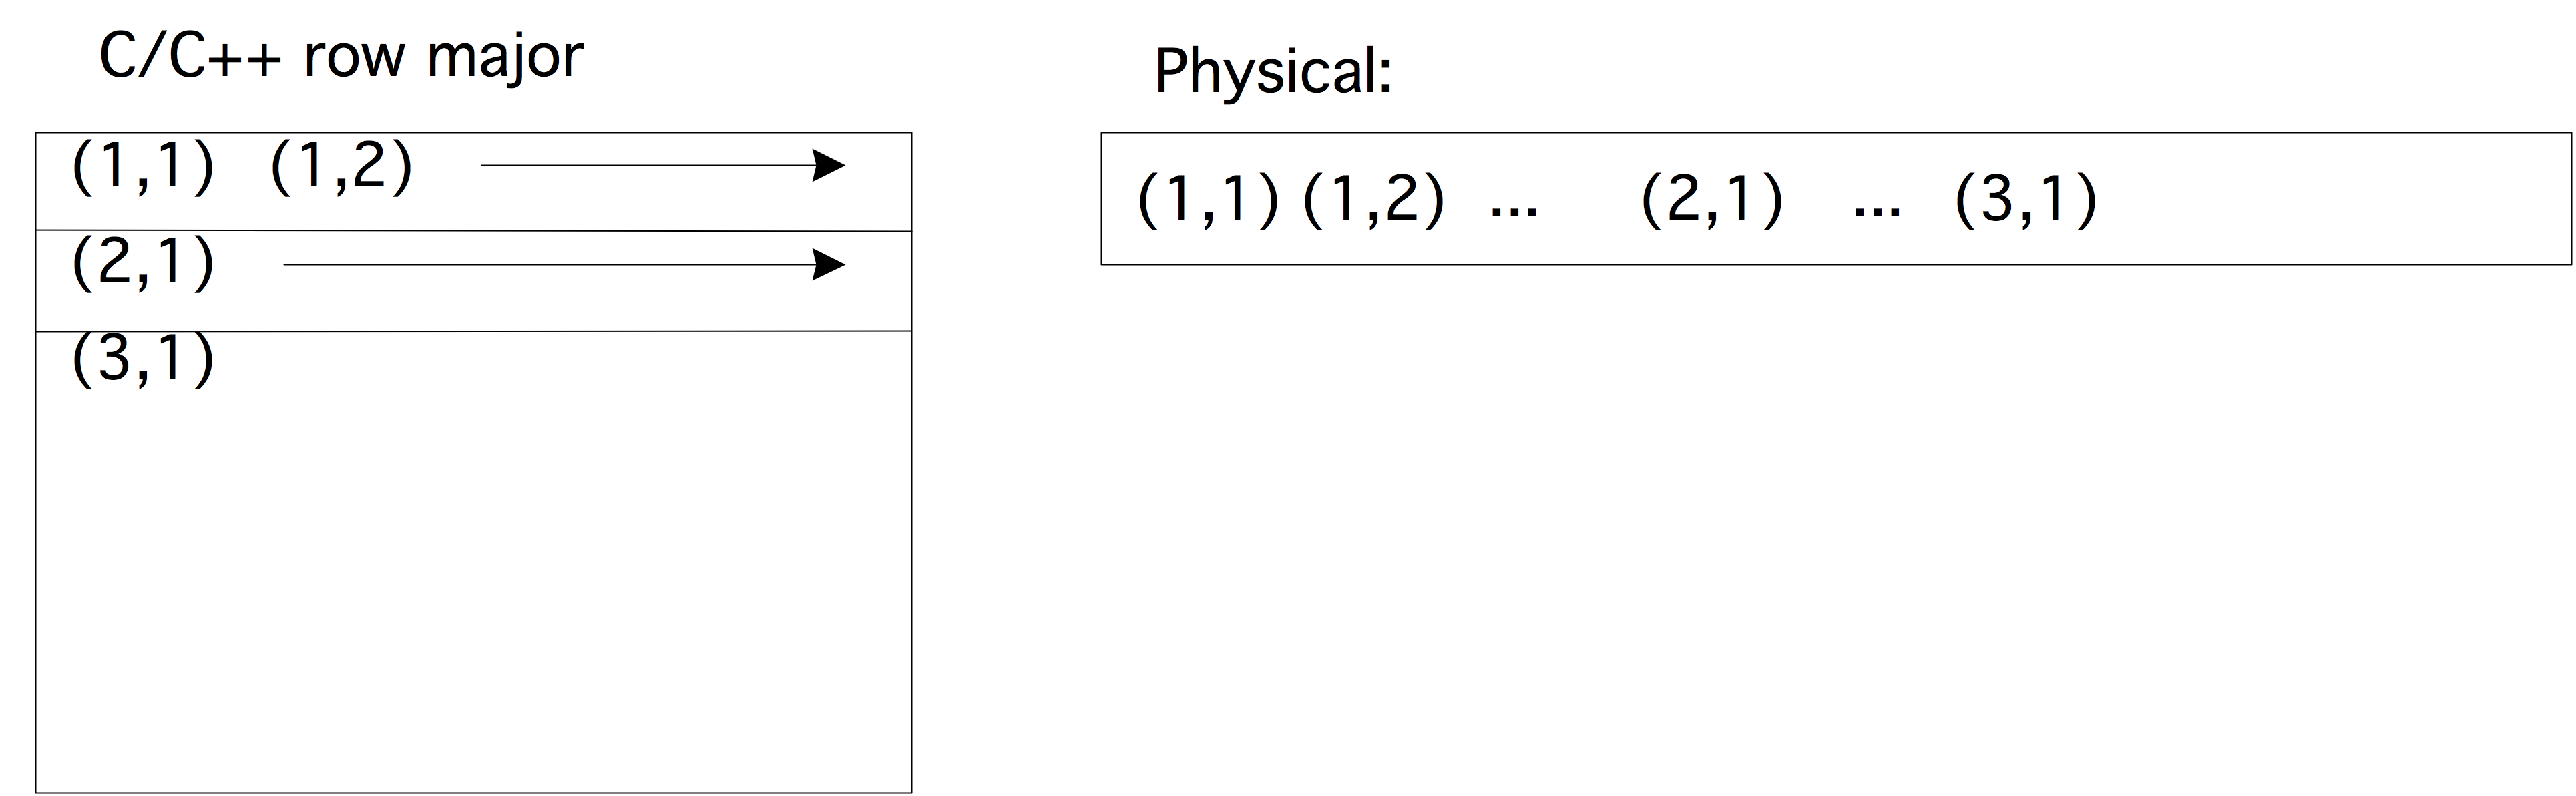
\includegraphics[scale=.1]{arrayc}

\Level 1 {Memory layout}

Puzzling aspects of arrays, such as which dimensions need to be
specified and which not in a function call, can be understood by
considering how arrays are stored in memory.
The question then is how a two-dimensional (or higher dimensional)
array is mapped to memory, which is linear.
\begin{itemize}
\item A one-dimensional array is stored in contiguous memory.
\item A two-dimensional array is also stored contiguously, with first
  the first row, then the second, et cetera.
\item Higher dimensional arrays continue this notion, with contiguous
  blocks of the highest so many dimensions.
\end{itemize}

As a result of this, indexing beyond the end of a row, brings you to the
start of the next row:
%
\verbatimsnippet{arraywrap}

We can now also understand how arrays are passed to functions:
\begin{itemize}
\item The only information passed to a function is the address of the
  first element of the array;
\item In order to be able to find location of the second row (and
  third, et cetera), the subprogram needs to know the length of each
  row.
\item In the higher dimensional case, the subprogram needs to know the
  size of all dimensions except for the first one.
\end{itemize}

\Level 0 {Exercises}

\begin{exercise}
  \label{ex:even-index}
  Given a vector of integers, write two loops;
  \begin{enumerate}
  \item One that sums all even elements, and
  \item one that sums all elements with even indices.
  \end{enumerate}
  Use the right type of loop.
\end{exercise}

\begin{exercise}
  Program \indexterm{bubble sort}: go through the array comparing
  successive pairs of elements, and swapping them if the second is
  smaller than the first. After you have gone through the array, the
  largest element is in the last location. Go through the array again,
  swapping elements, which puts the second largest element in the
  one-before-last location. Et cetera.
\end{exercise}

\begin{block}{Pascal's triangle}
  \label{sl:pascal-def}
  \small
  \indexterm{Pascal's triangle} contains binomial coefficients:
{\scriptsize
\begin{verbatim}
Row    1:                     1
Row    2:                   1   1
Row    3:                 1   2   1
Row    4:               1   3   3   1
Row    5:             1   4   6   4   1
Row    6:           1   5  10  10   5   1
Row    7:         1   6  15  20  15   6   1
Row    8:       1   7  21  35  35  21   7   1
Row    9:     1   8  28  56  70  56  28   8   1
Row   10:   1   9  36  84 126 126  84  36   9   1
\end{verbatim}
}
where \[ p_{rc} = \begin{pmatrix} r\\c \end{pmatrix} = \frac{r!}{c!(r-c)! }. \]
The coefficients can be computed from the recurrence
\[ p_{rc} = 
\begin{cases}
  1&c\equiv 1\vee c\equiv r\\
  p_{r-1,c-1}+p_{r-1,c}
\end{cases}
\]
(There are other formulas. Why are they less preferable?)
\end{block}

\begin{exercise}
  \label{ex:pascal-ex}
  \small
  \begin{itemize}
  \item 
    Write a class \n{pascal} so that \n{pascal(n)} is the object
    containing $n$~rows of the above coefficients. Write a method
    \n{get(i,j)} that returns the $(i,j)$ coefficient.
  \item
    Write a method \n{print} that prints the above display.
  \item First print out the whole pascal triangle; then:
  \item
    Write a method \n{print(int m)} that prints a star if the
    coefficient modulo~$m$ is nonzero, and a space otherwise.
\begin{verbatim}
          *
         * *
        *   *
       * * * *
      *       *
     * *     * *
    *   *   *   *
   * * * * * * * *
  *               *
 * *             * *
\end{verbatim}
  \end{itemize}
\end{exercise}
\begin{block}{Exercise continued}
  \label{sl:pascal-ex-contd}
  \begin{itemize}
  \item
    The object needs to have an array internally. The easiest solution
    is to make an array of size $n\times n$.
  \item Your program should accept:
    \begin{enumerate}
    \item
      an integer for the size
    \item any number of integers for the modulo; if this is zero, stop,
      otherwise print stars as described above.
    \end{enumerate}
  \end{itemize}
\end{block}


\begin{exercise}
  \label{ex:pascal-ey}
  Extend the Pascal exercise:\\
  Optimize your code to use
  precisely enough space for the coefficients.
\end{exercise}

\begin{exercise}
  A knight on the chess board moves by going two steps horizontally or
  vertically, and one step either way in the orthogonal
  direction. Given a starting position, find a sequence of moves that
  brings a knight back to its starting position. Are there starting
  positions for which such a cycle doesn't exist?
\end{exercise}

\begin{exercise}
  From the `Keeping it REAL' book, exercise 3.6 about Markov chains.
\end{exercise}

\begin{figure}[ht]
  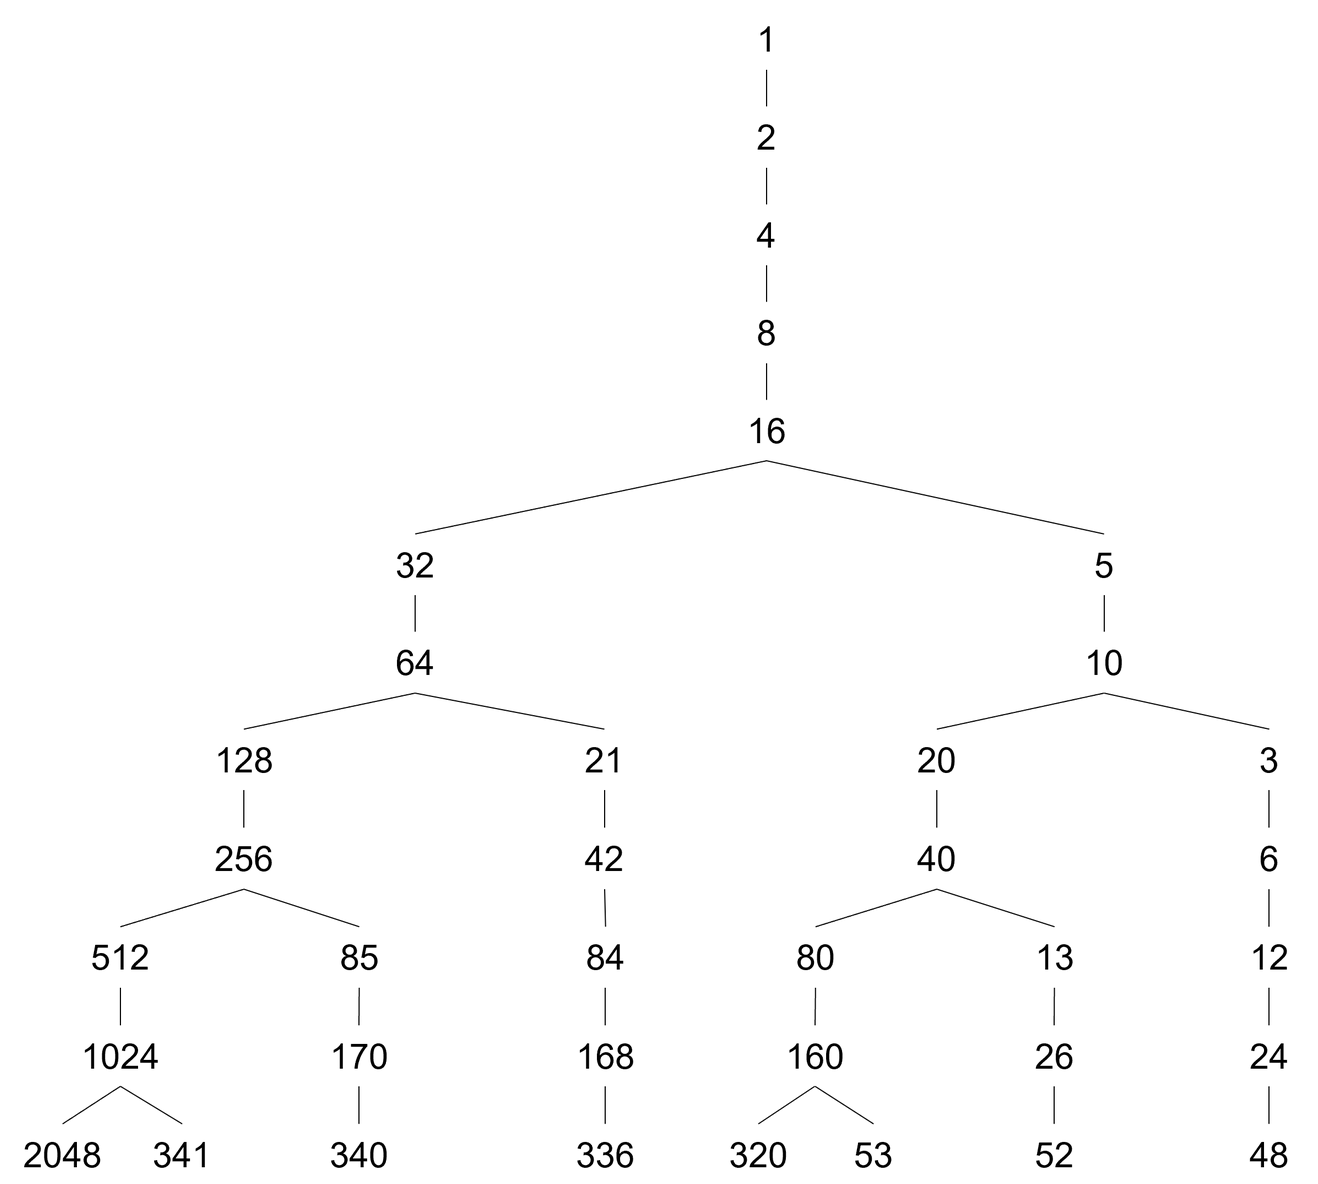
\includegraphics[scale=.5]{collatz-tree}
  \caption{The `Collatz tree'}
  \label{fig:collatz-tree}
\end{figure}

\begin{exercise}
  Revisit exercise~\ref{ex:collatz},
  and generate the `Collatz tree' (figure~\ref{fig:collatz-tree}):
  at level $n$ (one-based counting)
  are the numbers that in $n-1$ steps converge to~1.

  Read in a number $n$ and print the first $n$ rows,
  each row on a new line, with the numbers separated by spaces.
\end{exercise}

\ifIncludeAnswers
\else
\endinput
\fi

\Level 0 {Homework discussions}

\Level 1 {Pascal}
\label{sec:pascal-discussion}

\begin{multicols}{2}
  \scriptsize
  \lstset{basicstyle=scriptsize}
  \input pascal_discussion
  \lstset{basicstyle=footnotesize}
\end{multicols}
